\subsection{Erschütterungen}

\begin{frame}
\frametitle{Erschütterungsemissionen/-immissionen}
\begin{center}
 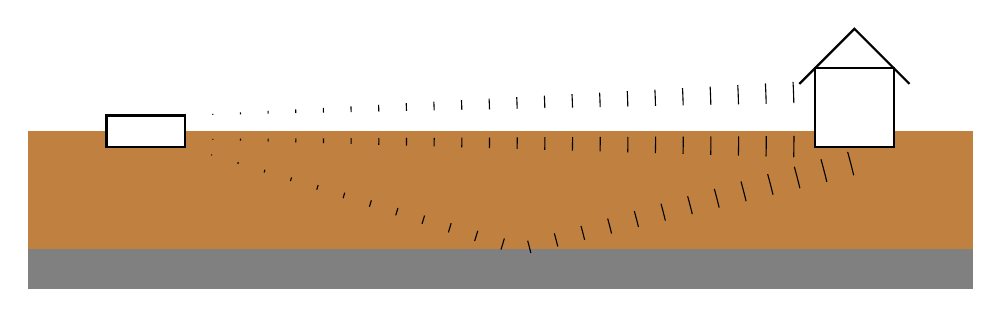
\begin{tikzpicture}
 \fill[color=brown] (-6,-1.5) rectangle (6, 0);
 \fill[color=gray] (-6,-2) rectangle (6,-1.5);
 \draw[thick, fill=white] (-5,-0.2)  rectangle (-4, 0.2);
 \draw[thick, fill=white] ( 4,-0.2)  rectangle ( 5, 0.8);
 \draw[thick] (3.8, 0.6) -- (4.5, 1.3) -- (5.2, 0.6);
 \draw[decorate,decoration={expanding waves, angle=1}] (-4, 0.2) -- (4, 0.5);
 \draw[decorate,decoration={expanding waves, angle=1}] (-4,-0.1) -- (4,-0.2);
 \draw[decorate,decoration={expanding waves, angle=1}] (-4,-0.2) -- (0.25,-1.5) -- (4.5,-0.4);
\end{tikzpicture}

\end{center}
\begin{description}[leftmargin=!,labelwidth=1mm]
\item[Quellen] Verkehr, Bauarbeiten, Maschinen, Naturereignisse
\item[Übertragungsweg] Boden (Dämpfung, Reflexion, Transmission) und Luft (hier nicht betrachtet) 
\item[Empfänger] Gebäude(teile), Lebewesen, Geräte
\end{description}
\end{frame}


\begin{frame}
\frametitle{Erschütterungsemission {\normalsize durch Verkehr}}
Logarithmische Darstellung der Partikelgeschwindigkeit \cite{studer2008bodendynamik}
\begin{equation*}
 L_v=\mathrm{dB}(v)=20\log\left(\frac{v}{v_\mathrm{ref}}\right)
\end{equation*}
bezogen auf den Referenzwert $v_\mathrm{ref}=\SI{1e-6}{\milli\metre\per\second}$ (ISO 1683).
Damit folgende Übertragungsverluste und -verstärkungen
\begin{equation*}
L_\mathrm{immision}=L_\mathrm{emision}
\underbrace{-\Delta L_{v,\mathrm{geom}}-\Delta L_{v,\mathrm{mat}}- \Delta L_{v,\mathrm{refl}}}_{\text{Verluste im Übertragungsmedium}}
\underbrace{-\Delta L_{v,\mathrm{koppl}}-\Delta L_{v,\mathrm{empf}}}_{\text{Verluste/Verst. am Empfänger}}
\end{equation*}
TODO fig 5.6 \cite{studer2008bodendynamik}
\end{frame}


\begin{frame}
\frametitle{Erschütterungsemission {\normalsize durch Bauarbeiten}}
Speziell für Spreng- und Rammerschütterungen \cite{studer2008bodendynamik} ist die Messung an der Quelle schwierig, deswegen wird die eingebrachte Energie als Kenngröße benutzt
\begin{equation*}
 v=cW^\alpha r^\beta.
\end{equation*}
TODO Details

Maschinen sind Punktequellen und werden nach der gleichen Formel geschätzt \cite{studer2008bodendynamik}.
\end{frame}


\begin{frame}
\frametitle{Erschütterungseinwirkung}

TODO fig 5.11 \cite{studer2008bodendynamik} % Belästigung (subjektiv) vor Schädigung
TODO fig 5.12 \cite{studer2008bodendynamik} % Messort entscheidend

\end{frame}

\begin{frame}
\frametitle{Erschütterungseinwirkung {\normalsize auf Bauwerke}}
Deutschland DIN 4150-3 (1999) Erschütterungen im Bauwesen, Einwirkungen
auf bauliche Anlagen.
 VDI 2716 (2001 mit Berichtigungen 2003) Luft- und Körperschall
bei Schienenbahnen des öffentlichen Personennahverkehrs

Kennwert Partikelgeschwindigkeitsvektor

Schweiz
Häufigkeitsklassen: gelegentlich, häufig, permanent
Empfindlichkeitsklassen: sehr wenig/wenig/normal/erhöht empfindlich 
Richtwerte
\cite{studer2008bodendynamik}

\end{frame}


\begin{frame}
\frametitle{Erschütterungseinwirkung {\normalsize auf Menschen}}
Kriterien \cite{studer2008bodendynamik}
Deutschland  DIN 4150-2 (1999) Erschütterungen im Bauwesen, Einwirkungen
auf Menschen in Gebäuden. DIN Deutsches Institut für Normung
VDI 2057 (2002) Einwirkung mechanischer Schwingungen auf den
Menschen, Blatt 1, 2 und 3, VDI Verein Deutscher Ingenieure

Schwingung und (primär, sekundär) Schall (unterschiedlich gewichtet in Normen)
TODO fig 5.16 \cite{studer2008bodendynamik}
\end{frame}


\begin{frame}
\frametitle{Erschütterungseinwirkung{\normalsize auf Geräte}}
ISO 8569:1996 Mechanical vibration and shock – Measurement and evaluation of
shock and vibration effects on sensitive equipment in buildings
\cite{studer2008bodendynamik}

\end{frame}


\begin{frame}
\frametitle{Erschütterungsreduktion}
\cite{studer2008bodendynamik}

Quelle: optimiertes Sprengschema, Maschinenfundamente, Unterschottermatten, Zusatzmassen/fundament

Übertragungsmedium: Schlitze TODO fig 6.19

Empfänger: Auflagerung/Fundament, Schwingungstilger (2dof)
\end{frame}


\begin{frame}
\frametitle{Beispiel}
4.3.3 \cite{haupt1986bodendynamik}
\end{frame}


